%% Change "letterpaper" in the following line to "a4paper" if you must.

\documentclass[10pt,letterpaper]{article}

\usepackage{cogsci}

%\cogscifinalcopy % Uncomment this line for the final submission 


\usepackage{pslatex}
\usepackage{apacite}
\usepackage{float}
\usepackage{graphicx}
\usepackage{xcolor}
\usepackage{multirow}
% \usepackage{gb4e}
\graphicspath{ {./images/} }
% \usepackage[noabbrev]{cleveref}

\newcommand{\tableref}[1]{Table~\ref{#1}}
\newcommand{\eref}[1]{(\ref{#1})}
\newcommand{\figref}[1]{Fig.~\ref{#1}}
\newcommand{\expref}[1]{Exp.~#1}

\definecolor{Pink}{RGB}{255,50,170}
\newcommand{\jd}[1]{\textcolor{Pink}{[jd: #1]}} 

\definecolor{Blue}{RGB}{0,50,255}
\newcommand{\stp}[1]{\textcolor{Blue}{[sp: #1]}} 


\title{The role of production expectations in  visual world paradigm linking hypotheses}
 
\author{}


\begin{document}

\maketitle


\begin{abstract}

While widely used in psycholinguistics, the linking hypothesis for eye movements in the visual world paradigm is still poorly understood. Recent work on linking hypotheses for referential tasks in particular has found mixed support for the \emph{Referential Belief Link}: that the proportion of looks to a referent in a time window reflects participants' degree of belief that the referent is the intended target in that time window. Here we test the hypothesis that participants' expectations for the utterances observed in an experiment modulate the extent to which the Referential Belief Link holds. This hypothesis is motivated by a simple idea: when utterances are unexpected, listeners engage in additional reasoning to make sense of the observed signal. In a re-analysis of a previous eye movement and incremental decision task dataset, in conjunction with two novel production experiments, we find that the more surprising an observed utterance is, the smaller the correlation between explicit and implicit beliefs is. We discuss the importance of participants' production expectations in research using the visual world paradigm.\\
\textbf{Keywords:} psycholinguistics; experimental pragmatics; scalar implicature; linking hypothesis; visual world paradigm; eye-tracking

\end{abstract}

\section{Introduction}
The visual world paradigm (VWP) is widely used in psycholinguistics. In the VWP, participants' eye movements are recorded as they listen to unfolding speech while viewing visual scenes like that in \figref{fig:display}.  Research using the VWP has had tremnedous success in furthering our understanding of phonetic, lexical, syntactic, prosodic, semantic, and pragmatic processing  \cite{tanenhaus1995,Allopenna1998,altmann1999,clayards2008,SedivyEtAl1999:Achieving-Incremental-Semantic-,huang2009,kurumada2014}. %LeffelXiangKennedy2016:Imprecision-is-Pragmatic-,}

The VWP is popular for good reason: eye movements can be interpreted as an indicator of attention that is closely time-locked to the linguistic signal. Language can guide eye movements to a region of interest in a display within 200 ms \cite{Allopenna1998}. By sampling an x/y coordinate every few milliseconds, researchers thus obtain a temporally fine-grained record of participants' language-directed attention over the course of an unfolding utterance. This property has been particularly useful in resolving questions regarding the time-course of online language processing, which typically cannot be addressed using offline measures like forced choice, truth-value judgments, or even more coarse-grained temporal measures like response times from button presses. 
% Notable VWP findings that could not have been obtained with more coarse-grained measures include the diverse insights that visual context is rapidly integrated into syntactic structure assignment \cite{tanenhaus1995}, %,chambers2004}, 
% that words are processed incrementally and listeners maintain uncertainty about past input \cite{Allopenna1998,clayards2008}, and that listeners anticipate upcoming linguistic material based on selectional restrictions and rapid pragmatic reasoning \cite{altmann1999,SedivyEtAl1999:Achieving-Incremental-Semantic-}. 



Despite its general success, the linking hypothesis for the VWP -- that is, how to link observed eye movements to the underlying mental processes that generate them -- is still poorly understood \cite{SalverdaTanenhaus2017:The-Visual-World-Paradigm, tanenhaus2000eye, Allopenna1998, magnuson2019fixations}. The problem of how to interpret eye movement patterns  is compounded by the fact that the VWP is used for vastly different tasks \cite<for an overview, see>{Huettig2011}. 

In this work we focus on active referential tasks, in which participants' goal is to identify and select the speaker's intended referent. In such tasks, eye movements are assumed to reflect listeners' active search for or belief in the referent. A way of formalizing this is the \emph{Referential Belief Link} \cite{DegenEtAl2021}, first proposed by \citeA{Allopenna1998}:
\begin{equation}
p_{\textrm{empirical}}(r|u) \propto p_{\textrm{belief}}(r = \textrm{target}|u)
\end{equation}

This captures the idea that the empirical proportion of looks $p_{\textrm{empirical}}$ to a referent $r$ in a time window in response to a (possibly partial) utterance $u$ reflects participants' degree of belief $p_{\textrm{belief}}$ that $r$ is the intended target.\footnote{As \citeA{DegenEtAl2021} caution, the assumption of proportionality may be too strong. A weaker version is that $p_{\textrm{empirical}}$ is monotonically increasing in $p_{\textrm{belief}}$.}

This linking hypothesis implicitly underlies much work in the VWP using referential tasks and is thus important to test explicitly. Recent work doing so has found mixed support for it \cite{QingLD2018, DegenEtAl2021}. In these studies,  previous eye-tracking datasets were re-analyzed with respect to how closely proportions of eye movements to a referent within a time window correlated with explicitly elicited referential beliefs \cite{QingLD2018, DegenEtAl2021}. Explicit referential beliefs were collected in an offline \emph{incremental decision task}
\cite<similar to gating tasks,>{Allopenna1998,KreissDegen2020}. In a re-analysis of an adjective processing dataset \cite{LeffelXiangKennedy2016:Imprecision-is-Pragmatic-}, \citeA{QingLD2018} found low or no correlations between explicit beliefs and eye movements (all $r \in [0.06, 0.46]$ in the theoretically relevant window of analysis). In contrast, the same methodology applied to a quantifier processing dataset \cite{sun2020} found high correlations \cite<all $r \in [0.79,0.96]$ in the theoretically relevant window of analysis, >{DegenEtAl2021}. 

What determines the observed variability in the extent to which the Referential Belief Link holds both across and within studies? \citeA{QingLD2018} propose an interesting hypothesis, motivated by the idea that there is a tradeoff between \emph{exploration} and \emph{exploitation}: when participants are less familiar with the objects in the scene and the ways of referring to them, eye movements might serve a more exploratory purpose, i.e., to establish the  referent options and how speakers might refer to them. In contrast, with more familiarity with possible referents and ways of referring to them, participants might have more resources available for exploiting their signal-driven beliefs.

A prediction of this speculative idea is that if listeners observe a less expected utterance, they will need to explore the scene more, e.g., to evaluate which possible referents are compatible with the utterance, and hence the correlation between proportions of looks and explicit referential beliefs should be weaker. In contrast, if listeners hear a more expected utterance, they can directly exploit the signal, and hence  the correlation between proportions of looks and beliefs should be stronger. \citeA{QingLD2018} found preliminary evidence for this prediction: while the adjectivally modified referring expressions used in the original study were rarely produced naturally in a free production experiment, the single condition in which explicit beliefs were predictive of eye movements was also the condition in which the observed referring expressions had a non-zero (albeit still very low) probability of being produced naturally.



Here we report a direct test of the hypothesis that listeners' expectations for the utterances observed in a visual world eye-tracking  experiment modulate the extent to which the Referential Belief Link holds. We do so by testing the extent to which participants' quantifier production expectations, estimated in two free production tasks, predict the correlation between implicit and explicit beliefs as measured in the quantifier processing datasets collected by \citeA{sun2020} and \citeA{DegenEtAl2021}.






\begin{figure}[h]
\centering
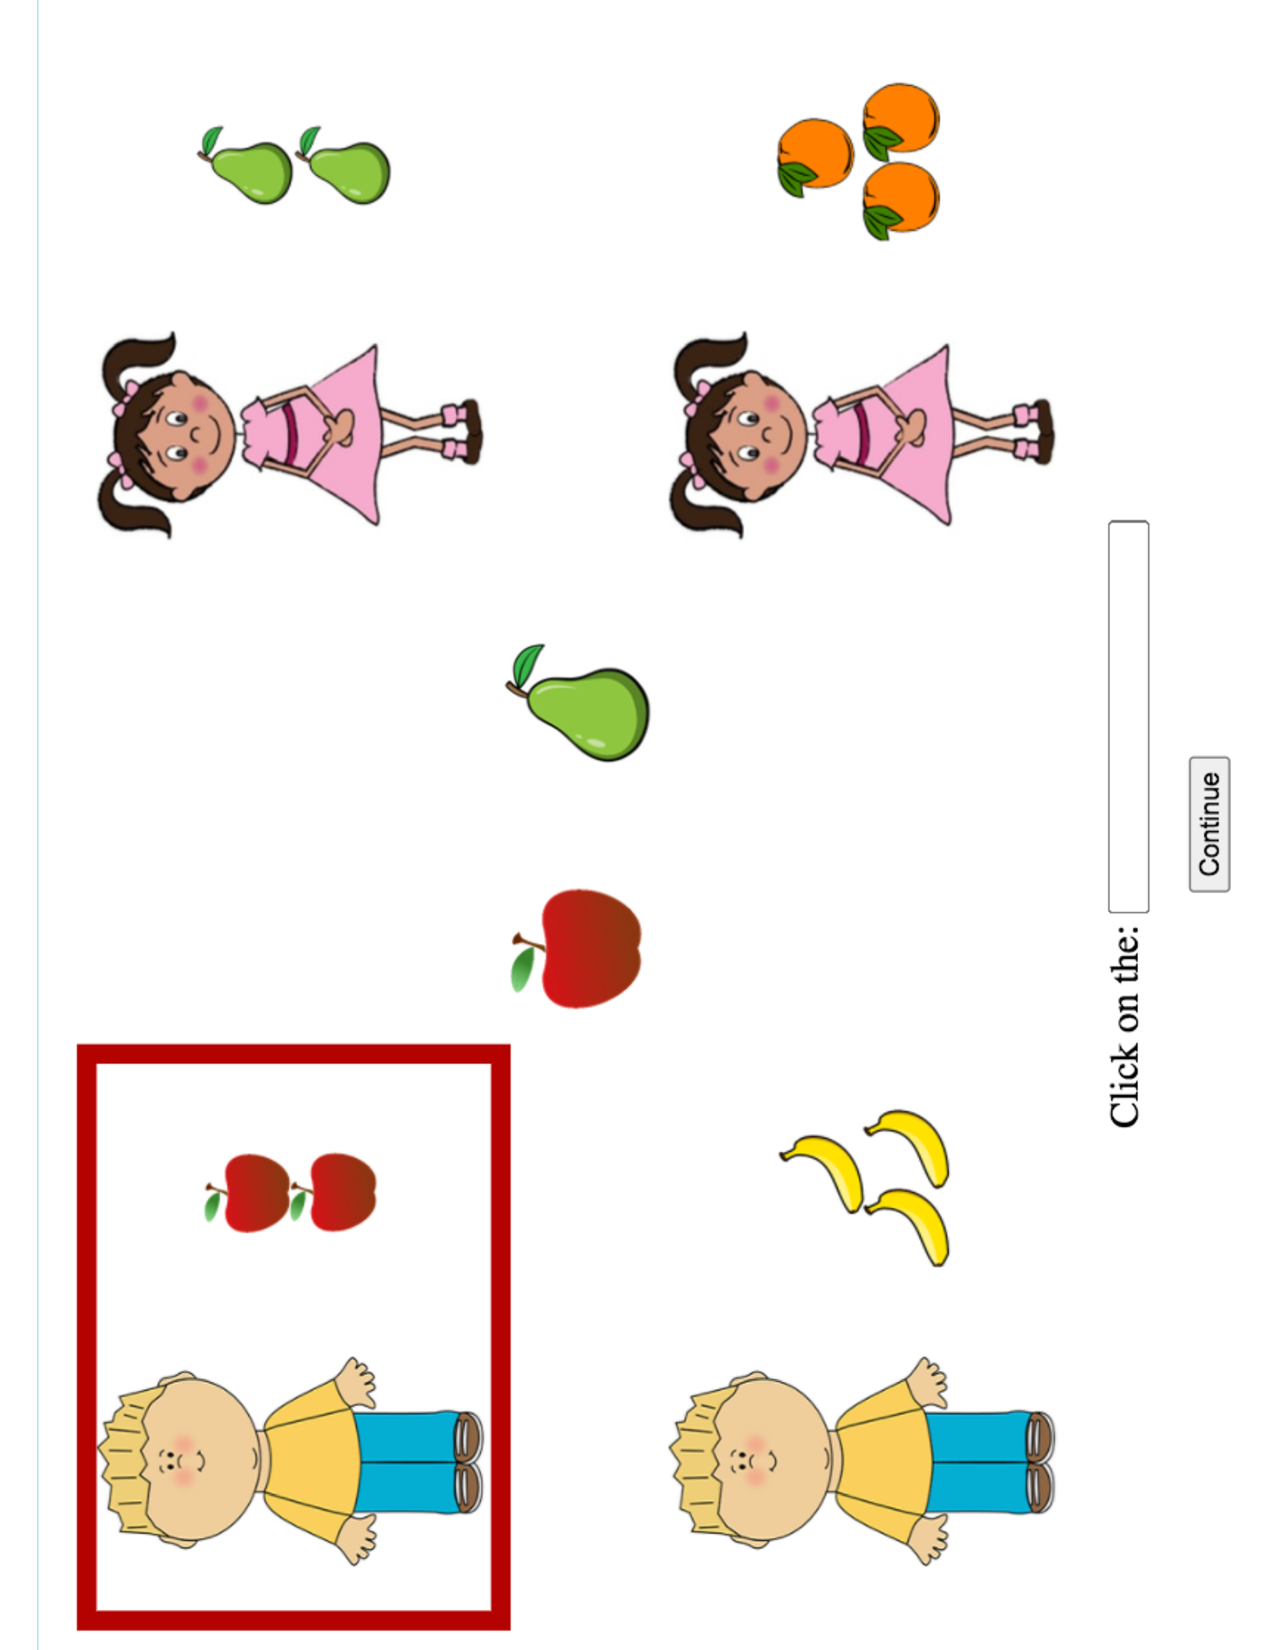
\includegraphics[width=.35\textwidth,angle=270]{images/instructionImage}
\caption{Example display in our written production experiments. The same display types were used in \citeA{sun2020}'s eye-tracking Experiment 3 without the red border and text field prompt, paired with instructions like `Click on the boy with some of the apples.'}
\label{fig:display}
\end{figure}

\section{Research strategy and test domain}

We used the displays of \citeA{sun2020} (see \figref{fig:display}) to elicit natural referring expressions in two written free production tasks. This allowed us to compute a proxy measure for participants' quantifier production expectations in the original experiment as   the surprisal of each quantifier in the two production tasks.\footnote{The use of surprisal rather than probability is motivated by ample evidence showing that processing effort as measured in reading times or in N400 amplitudes in ERP studies is linear in word surprisal, not  probability \cite{levy2008,smithlevy2013,frank2013word}.}
If production expectations modulate the strength of the Referential Belief Link, quantifier surprisal should predict the correlations between implicit referential beliefs measured via eye movements in the VWP \cite{sun2020} and  explicit referential beliefs elicited in an incremental decision task \cite{DegenEtAl2021}.

We briefly describe the design of the original comprehension studies before introducing our novel production studies and main analysis.

\subsubsection{Sun and Breheny (2020)} investigated the processing speed of quantifiers. Specifically they were interested in how: 1) pre-existing low-level associations between quantifiers and set sizes (e.g., the preference for the quantifier “all” with larger set sizes of target objects) affect quantifier processing speed, and 2) how the quantifier used affects processing speed, specifically whether certain quantifiers (e.g., “all” or “some”) require an additional process of verifying the relationship between referent target objects and other objects in the scene (what they called the `residue set' in the center of the display). In order to address these questions, their Experiment 3 manipulated the set size of the target objects (big (3 objects) or small (2 objects)) and the quantifier used to describe the objects (“all”, “some” or a number). Visual scenes (such as \figref{fig:display}) were shown with auditorily presented instructions of the form “Click on the $|$ GENDER $|$ that has QUANTIFIER $|$ of NAME’S $|$ NOUN $|$”. GENDER was a gender noun (``boy'' or ``girl'') referring to the target child, QUANTIFIER was one of four quantifiers (“all”, “some”, “two”, or “three”), NAME referred to 1 of 3 characters who were introduced in a background story at the start of the experiment, and NOUN was 1 of 12 target objects (4 kitchenware items, 4 stationary items, or 4 fruit). Thus, a participant who saw the display in \figref{fig:display} may have heard the instruction `Click on the boy who has some of Susan's apples.' Participants' eye movements were analyzed in different time windows: Baseline, Gender, Quantifier, Name, and Noun (separated by `$|$' in the example instruction above). 

The theoretical window of interest was the Quantifier window. They found that eye movements to the target increased most rapidly in the Quantifier window in response to number terms. Looks increased more slowly for ``all'' and ``some,'' modulated to some extent by set size, but participants rapidly looked to the residue set in response to these quantifiers, presumably for verification purposes.

\subsubsection{Degen et al. (2021)} assessed the Referential Belief Link by replicating  \citeA{sun2020} in an incremental decision task. They presented the original instructions in written rather than auditory form, but revealed them incrementally, one window at a time.\footnote{They collapsed the Name window into the Quantifier window because the name did not provide additional information about the target.} After the participant  made a guess about the target in one window, the text in the next window was revealed. They then calculated correlations between participants’ explicit beliefs (as measured by referent selections within a window) and proportions of looks to referents in \citeA{sun2020}. Overall, selection data in the Quantifier window was highly correlated with looking data (all $r >$ .78), thus supporting the linking hypothesis. Nevertheless, correlations displayed variability, suggesting the Referential Belief Link was not supported to the same extent across conditions.

\subsubsection{The present study}
In order to test whether participants’ expectations for observed quantifiers modulate the extent to which the Referential Belief Link holds, we implemented the design of the original studies as free production tasks. Quantifier surprisal was computed as the negative logarithm of the relative frequency of the quantifier  within a specific combination of \citeA{sun2020}’s conditions and windows -- i.e., a combination of the target object set size (big, small), quantifier condition (“all”, “some”, number),  gender of target child within a trial (boy, girl) and target noun within a trial (1 of the 12 objects): 

\smallskip
\begin{equation*}
\label{surprisal}
\textrm{surprisal(det)} = - \log_2 P(\textrm{det}) = - \log_2 \frac{\textrm{freq(det)}}{\textrm{freq(combination)}}
\end{equation*}

\smallskip

Because log(0) is undefined, if a particular quantifier was never produced, we re-assigned that quantifier a probability of 0.0001, resulting in a surprisal of $\sim$13.29.

We computed quantifier surprisal in two different production tasks. The ``purest" form of eliciting production would be to allow participants to produce referring expressions following `Click on the\dots' with no constraints whatsoever. However, this would have likely resulted in referring expressions without quantifiers. For example, the target boy in \figref{fig:display} can be referred to simply as `the boy with apples.' This is a problem for instance for eye-tracking studies using referring expressions with quantifiers to probe the speed with which scalar inferences are drawn \cite{huang2009,grodner2010,DegenT2016,sun2020}, since it is not clear that pragmatic reasoning about alternatives naturally unfolds in the face of pragmatically infelicitous utterances. A cooperative speaker who insists on using a quantifier should at least produce one that will allow the listener to rapidly identify the target -- here, vague quantifiers like ``some'' should be dispreferred compared to number terms \cite<especially with the small set sizes considered here, >{DegenTanenhaus2015,sun2020}. Despite the importance of utterance alternatives (and listeners' resulting  production expectations) in the computation of pragmatic meaning \cite{franke2014,Goodman2016,peloquin2016,DegenTanenhaus2015,DegenT2016,gotzner2016,sun2020}, little work has been done to estimate how likely the utterances are that researchers provide participants in eye-tracking experiments on quantifier processing. The current study thus also provides novel, principled estimates of quantifier surprisal in the types of contexts frequently used in experimental pragmatics studies.

As mentioned above, the most likely outcome of an entirely unconstrained production task is  no quantifier production at all. Given that listeners rapidly update their beliefs about likely utterances in response to exposure \cite{grodner2011,pogue2016,schuster2020}, it is likely that participants in eye-tracking studies, where the same utterance form is observed repeatedly, rapidly form local expectations about likely utterances. 

We thus ran two versions of the production task: one in which participants received no exposure to the original comprehension task -- allowing for an estimate of non-adaptive quantifier base rates -- and one in which participants first completed four comprehension trials from \citeA{DegenEtAl2021} -- allowing for locally adaptive estimates of quantifier rates.

\section{Experiment 1: free production without   comprehension trial exposure}

%In order to compute the surprisal of utterances in Exp.~3 of \citeA{sun2020}, we implemented their experiment as a free production task.

\subsection{Methods}
\subsubsection{Participants}
We recruited 51 native English speaking participants in the United States on Prolific. We excluded participants with overall $<95$\% accuracy, participants who answered with single word responses on $>50$\% of trials, and participants who did not produce target object nouns on $>50$\% of trials. These criteria led to no participant exclusions. %Participants were compensated for their time. 

\subsubsection{Materials and Procedure}
 We used the same design and materials as \citeA{sun2020} but changed the task.\footnote{Pre-registrations will be available on OSF. Experimental materials, data, and analysis scripts will be available on GitHub.} On each trial, participants told a fictional addressee to click on one of four children in a display by typing into a text box. The target child to communicate was indicated by a red border (see \figref{fig:display} for an example display).   


Each display contained 4 children with an assortment of objects (fruit, kitchenware, or stationary) in four corners of the screen. In the middle, there were extra objects that matched the children's objects. Participants were told that their task was to ``\emph{get another player to click on the child in the red box}'' by ``\emph{complete[ing] the sentence `Click on the\dots' by typing what [they] think should come next}.'' On each trial they were given the phrase ``Click on the'' followed by an empty text box into which they could type their answer. Two example sentences were given on the instruction pages: ``Click on the boy with two of the apples'' and ``Click on the boy with some of the apples''. These example sentences were included to encourage participants to give responses that could include quantifiers. We only gave two example sentences in order to minimize interference with natural quantifier production. Crucially, participants were not explicitly told that their answers had to match any particular format or be restricted in any way. Therefore they were free to produce any utterance they deemed appropriate. 

The experiment followed the design of Sun and Breheny (2020) and included 56 trials: 36 experimental trials, 12 filler trials, and 2 practice trials. Experimental trials were evenly split by whether  the target object set size was big (3 objects) or small (2 objects) and by whether participants in \citeA{sun2020} originally heard the instruction with the quantifier ``all'', ``some'', or a number (``two'' or ``three''). Targets were counterbalanced for the child's gender (boy or girl) and type of object the child had (fruit, kitchenware, or stationary; total of 12 unique objects).  

%The filler trials were likewise evenly split up across the boy/girl, big/small, and fruit/kitchenware/stationary dimensions. However, the filler trials only included target set sizes of 1 or 4 objects. 
There were two practice trials which were identical in procedure to the rest of the experiment. For consistency, the practice trial scenarios (sets of children and objects presented in the scene) were taken from Sun and Breheny's (2020) Exp. 3 practice trials. Experimental trial order was randomized.

%Participants were randomly assigned one of the three original stimuli lists \textcolor{green}{(FIGURE OUT WHAT THE EXACT DIFFERENCE IN THE LISTS WAS)} and the order of presentation of experimental/filler stimuli was randomized


\subsection{Results and discussion}


Trials were excluded from analysis if participants produced  an incorrect gender (n = 3),  an incorrect quantifier (n = 6), an incorrect target object noun (n = 17), no target object noun (n = 0), or a single word response (n = 0), resulting in the exclusion of  26 trials (1.5\%). We focus on the quantifier window as our main window of analysis.

Quantifiers in participants' productions were classified as belonging to the following categories: ``all'', ``some'', number (``two'' or ``three''), no quantifier, or other (e.g., ``most'', ``least'', ``both''). Individual surprisal values were calculated for each unique combination of noun (eraser, apple, \dots) and target set size (big, small).

\figref{fig:surprisalResults} shows the mean surprisal for each quantifier category. Of the quantifiers included in the original study, number terms were produced most frequently (1182 of the 1810 trials), yielding a very low surprisal of 0.6 (for both the big and small set size). Much less frequently produced was ``some'' (48 of the 1810 trials), yielding a relatively higher surprisal of 5.1 (for the big set size) and 6.2 (for the small set size). Perhaps most surprisingly, ``all'' was never naturally produced, leading to a very high surprisal value (at ceiling). Of note is that the second most preferred utterance type did not include a quantifier at all (e.g., ``Click on the boy with apples''). This confirms the intuition that using no quantifier at all to describe the target objects is among the most expected alternatives. All of the reported differences were supported by a mixed effects linear model predicting surprisal from dummy-coded fixed effects of quantifier (reference level: `some'), set size (reference level: `big'), and their interaction, with random by-noun intercepts. There were no significant set size effects (all $|t| < 1.5$).

%asteriks after figure makesit spread out over two columns
%.pdf ending is assumed

\begin{figure}[h]
\centering
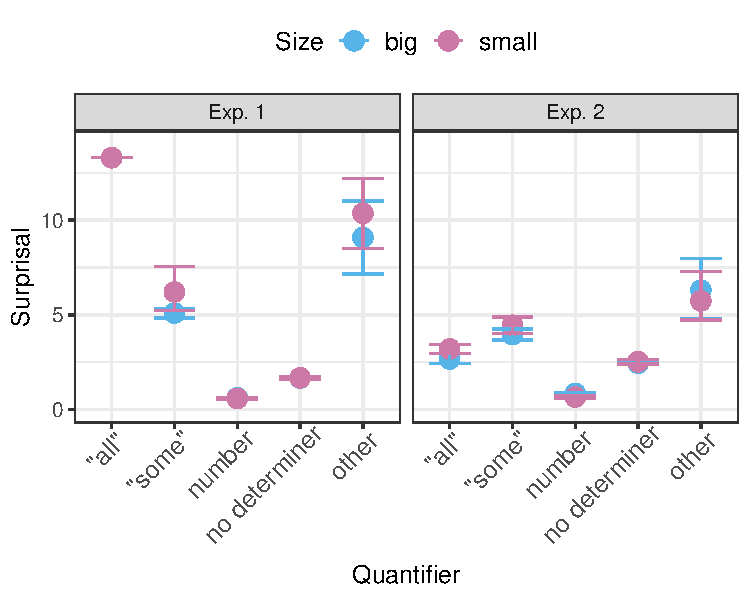
\includegraphics[width = 0.475 \textwidth]{images/det_surprisal_faceted}
\caption{Mean surprisal of quantifiers in Exps.~1 and 2. Error bars indicate 95\% bootstrapped confidence intervals. Values were calculated separately for the two different target object set sizes (big and small).}
\label{fig:surprisalResults}
\end{figure}

Overall, then, the instructions widely used in studies on pragmatic inferences based on quantifier use \cite{huang2009,grodner2010,DegenT2016,sun2020} are highly unexpected, raising a question about the generalizability of the results of these studies to contexts where non-number quantifiers are expected. However, as acknowledged above, listeners rapidly adapt to the updated statistics of their linguistic environments. Thus, a fairer estimate of quantifier production expectations might be obtained after brief exposure to the original comprehension task. This was the goal of Exp.~2.

% \jd{moved down from materials: }Their rates of use of gender, quantifiers, and nouns \textcolor{green}{dependency} were then used to calculate surprisal of instructions from the original SB2020 study.

% \begin{equation}
% P(\textrm{det} | \textrm{group}) = \frac{\textrm{\# of occurrences of a det within a group}} {\textrm{total \# of trials within a group}}
% \end{equation}
% \jd{we need to clean up both of these equations once i understand what a "group" is}


\section{Experiment 2: free production with comprehension trial exposure}
\subsection{Methods}
\subsubsection{Participants}
We recruited 51 native English speaking participants in the United States from Prolific. We excluded participants using the same criteria as in Exp. 1, which led to the exclusion of (n = 2) participants. %Participants were compensated for their time. 

\subsubsection{Materials and Procedure}
Exp. 2 was identical to Exp. 1 with the exception of 4 additional practice trials. The scenarios (children and objects shown on the screen) were identical to  trials in \citeA{DegenEtAl2021}'s incremental decision study. However, the target utterances were slightly modified so that all possible quantifiers from Sun and Breheny (2020) would be observed within the four trials. Participants were given an instruction of the form ``Click on the $|$ GENDER $|$ that has QUANTIFIER of NAME'S $|$  NOUN $|$'' incrementally and  selected what they believed to be the target of the utterance in each window (marked by `$|$'). %The utterances were given in the format of "Click on the GENDER who has quantifier of NAME's NOUN". 
The four practice trial sentences were: 

\begin{enumerate}
  \item Click on the boy that has two of Susan's apples.
  \item Click on the girl that has some of Susan's apples.
  \item Click on the boy that has three of Michael's scissors.
  \item Click on the girl that has all of Michael's rulers. 
\end{enumerate}

% \begin{exe}
%   \ex Click on the boy that has two of Susan's apples.
%   \ex Click on the girl that has some of Susan's apples.
%   \ex Click on the boy that has three of Michael's scissors.
%   \ex Click on the girl that has all of Michael's rulers. 
% \end{exe}


These practice trials were then followed by the instructions and practice trials from Exp.~1. %Therefore, participants had 4 extra cues that their answers could be in the above format and could include the quantifiers "two", "three", "some", and "all". Crucially, 
Participants were never explicitly told that their answers had to match any particular format or be restricted in any way. 

\subsection{Results and discussion}

Trials were excluded from analysis if participants produced  an incorrect gender (n = 2), an incorrect quantifier (n = 6), an incorrect target object noun (n = 16), no target object noun (n = 0), or a single word response (n = 13), resulting in the exclusion of 37 trials (2.1\%). 

Surprisal means by quantifier and target set size are shown in \figref{fig:surprisalResults}. Notably, while number was produced at similar rates as in Exp.~1 (1019 out of 1771 trials; surprisal = 0.86 (big set) and 0.67 (small set)), both ``some'' (106 out of 1771 trials; surprisal = 3.97 (big set) and 4.46 (small set)) and especially ``all'' (240 out of 1771 trials; surprisal = 2.68 (big set) and 3.21 (small set)) were produced more frequently. In fact, ``all'' was preferred over ``some'', though both were marginally more preferred with big than with small sets. As in Exp.~1, these differences were confirmed by mixed effects models. 

These results suggest that of the three quantifiers typically included in studies on scalar inferences -- ``all'', ``some'', and small number terms  like ``two'' and ``three'' -- only the number terms are naturally preferred to the unquantified alternative in production. Given the evidence that listeners have probabilistic  production expectations that  track the actual statistics of words in the world  \cite{levy2008, frank2013word}, the results suggest that only number terms are naturally expected in this paradigm. This may explain why number terms in such studies typically lead to  much faster target identification than either ``all'' or ``some'' \cite{huang2009,DegenT2016,sun2020}. 

\subsection{Correlation Analysis}
We can now assess the hypothesis that the extent to which the Referential Belief Link holds is modulated by participants' production expectations. To do so, we tested whether quantifier surprisal is a predictor of the correlation between implicit and explicit beliefs as reported by \citeA{DegenEtAl2021} for the quantifier window of \citeA{sun2020}.\footnote{We could have  run this same analysis in other time windows if there was any variability in word surprisal in those windows, but there wasn't. Surprisal values were close to zero in the gender window (because participants almost always produced the expected gendered noun ``girl'' or ``boy''), and zero in the noun window (because participants always produced the expected noun).} 

%by how surprisal modulates the linking hypothesis, we calculated the surprisal of seeing each word in SB2020’s original exp. 3 stimuli. We calculated the surprisal of the words found in the gender, quantifier, and noun windows. 

To this end we ran two linear models that predicted the quantifier window correlations (computed at the level of unique combinations of quantifier, target set size, and target child gender) from the surprisal values obtained in Exps.~1 and 2, respectively.
%\stp{"from the surprisal values obtained in Exps. 1 and 2, respectively". This is not technically true. We ran these models on the surprisal values we obtained for the correlation analysis (i.e. the one split up by condition-size-gender) and not the experimental surprisal values (i.e. the ones split up by determiner Used - size - noun)}\jd{yes, but we got all the data in exps1 and 2}
\figref{fig:detSurprisalCorr} shows Quantifier window correlations against surprisal values.  

Surprisal as estimated in Exp.~1 was a significant predictor of the correlations ($\beta$=-0.006, $SE$=0.001, $t$=-4.16, $p<$.001), as was surprisal as estimated in Exp.~2 ($\beta$= -0.039, $SE$=0.004, $t$=-9.65, $p<$.0001). However, Exp.~2 surprisal was a better predictor of correlations than Exp.~1 surprisal, as evidenced in twice the variance explained (Exp.~1 adjusted $R^2 = 0.27$, Exp.~2 adjusted $R^2 = 0.55$). This improvement is largely driven by the difference in estimates for ``all'' surprisal and provides indirect evidence that listeners indeed rapidly formed experiment-specific quantifier expectations. 

These results thus suggest that the more expected the quantifier was in the original experiment, the more participants' explicit beliefs predicted implicit beliefs, i.e., the more strongly the Referential Belief Link held.


%\textcolor{blue}{Add something to make this previous analysis flow into the next one (where we give the final correlation values. Should this analysis go after the two paragraphs below? Or should we get rid of the paragraphs below all together and move the final correlation values up here?}
%\jd{we don't need}

% \subsubsection{Degen et al. 2021}
% In order to compare surprisal values with the correlations from Degen et al. 2021, we replicated the correlations from Degen et al. 2021. However, rather than just calculating the correlations between clicks of a target and looks to the target based on condition (all, some, and number) and target object set size (big and small), we further split these correlations up by target child gender (boy vs. girl).

% \subsubsection{Experiment Comparison for quantifiers}
% The quantifiers of interest from the original study were: ``all'', ``some'', or a number (``two'' or ``three''). We first grouped the trials by the three experimental conditions of Sun and Breheny (2020), which determined which of the three quantifier types the participant heard. To match the original contexts within which participants heard these quantifiers, we grouped the trials by target object set size (big vs. small) and gender of target child (boy vs. girl). We then calculated surprisal within each of these condition-size-gender groupings using the calculation given in the Research strategy and test domain Section \textcolor{green}{link to section name}. The comparison between the correlations from Degen et al. 2021 and the gender surprisal values are given in \figref{fig:detSurprisalCorr}.
% We then computed the Pearson's correlation coefficient between the correlations from Degen et al. 2021 and the computed surprisal values for the quantifier window. Correlations between surprisal and correlations from Degen et al. 2021 for both experiment 1 ($Corr =$ -0.54, $p<$ .001) and experiment 2 ($Corr =$ -0.74, $p<$ .001) were found to be significant. However, the correlation for experiment 2 was found to be higher. \textcolor{blue}{Discuss what this means}

% \textcolor{green}{Go through and standardize "Experiment 1" versus "Exp. 1"}

% \textcolor{blue}{make sure that prose match the new updated model values}

\begin{figure}[htbp]
\centerline{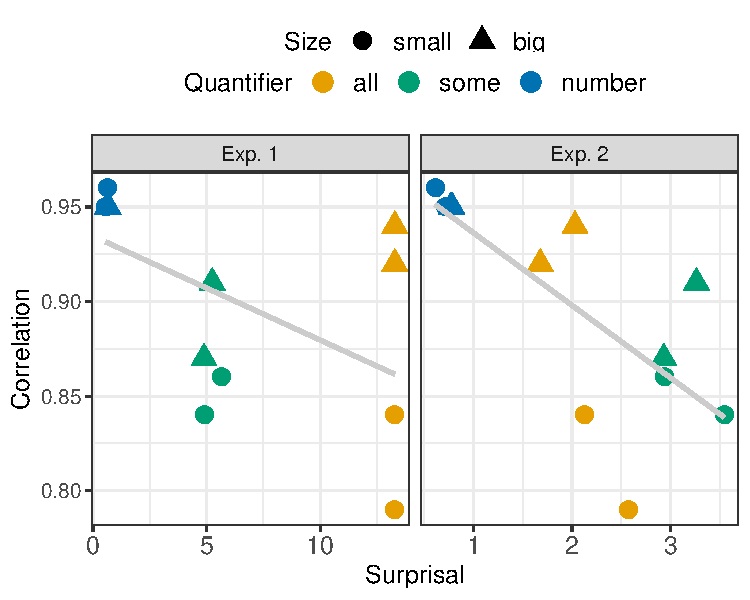
\includegraphics[width = 0.475 \textwidth]{images/surprisal_correlation.pdf}}
\caption{Correlation between implicit and explicit beliefs in the quantifier window of \citeA{sun2020} and \citeA{DegenEtAl2021} against quantifier surprisal. Gray line indicates regression line. Surprisal was calculated over combinations of quantifier, target object set size, and target child gender.}
\label{fig:detSurprisalCorr}
\end{figure}

\subsection{General Discussion}

Despite numerous attempts at shedding light on the issue of how to link observed eye movements to the underlying mental processes that generate them \cite{SalverdaTanenhaus2017:The-Visual-World-Paradigm, tanenhaus2000eye, Allopenna1998, magnuson2019fixations}, linking hypotheses for the visual world paradigm are still underdeveloped. In this work we tested a particular hypothesis about why a frequently implicitly assumed linking hypothesis -- the Referential Belief Link -- appears to variably hold across and even within studies. We found that the extent to which the Referential Belief Link holds for the quantifier processing dataset of \citeA{sun2020} was modulated by participants' likely quantifier production expectations. This result dovetails with the result previously reported by \citeA{QingLD2018} and \citeA{DegenEtAl2021} that correlations between implicit and explicit beliefs increased across subsequent time windows, as participants presumably became more certain about the intended target.


While we consider this work a promising first step towards understanding the applicability of linking hypotheses in the VWP, we hasten to list the caveats of this work. First, while we have shown that quantifier surprisal predicted the correlation between implicit and explicit beliefs, we have not yet provided a cognitive model of eye movements in the visual world. In this respect,  linking hypotheses for eye-tracking during reading are somewhat better developed  \cite<e.g., >{bicknell2010}.\footnote{\citeA{bicknell2010} spell out a computational model of eye movement control during reading in which eye movement
decisions are made to obtain (possibly noisy) visual information, which the reader uses in Bayesian inference about the form and structure of the sentence. It is an interesting question to what extent insights from the reading literature might be applied to the visual world.} A step in this direction for the visual world might be to  use  surprisal as a parameter that toggles between explicit referential beliefs and random looking; or between referential beliefs and structured looking. One reason for  structured looking is given by \citeA{sun2020}'s study: participants surprised by the use of ``some'' or ``all'' did not look randomly at objects in the display, but instead looked to the residue set for verification that the observed quantifier correctly applies to the target set under consideration. 


Further, the current work is limited to  referential tasks, i.e., tasks in which the listener's goal is to identify and select the speaker's intended referent. Other tasks, e.g., certain passive listening tasks which have been shown to elicit predictive eye movements \cite{altmann1999}, will require a different linking hypothesis.

This work raises interesting questions regarding the role of production expectations in  experimental pragmatics comprehension studies. The fact that referential beliefs  elicited in an offline selection task were more weakly correlated with  the eye movement data precisely in those conditions where the observed quantifier was more surprising, provides support for accounts of pragmatic inference that ascribe delays in target identification not to inference computation cost per se \cite{bott2004,huang2009,huang2018}, but to additional sense-making processes that must be engaged when observing surprising language \cite{DegenTanenhaus2015, sun2020}. Future work should further distentangle the relative costs contributed by inference computation vs.~additional sense-making processes. 

Finally, we have shown here that there is good reason to believe that production expectations play an important role in visual world paradigm linking hypotheses. Future work should assess the generalizability of this finding by extending the investigation across a wider set of contexts and linguistic forms.



\bibliographystyle{apacite}

\setlength{\bibleftmargin}{.125in}
\setlength{\bibindent}{-\bibleftmargin}

\bibliography{bibliography}


\end{document}
